%% SIGCSE Virtual 2026 — CER Track
%% 6 body pages + 1 reference page
%% ACM sigconf, double-column, US Letter
%% Double-anonymous: author blocks anonymized for submission

\documentclass[sigconf,anonymous]{acmart}

%% ── Packages ──────────────────────────────────────────────────────────────
\usepackage{booktabs}
\usepackage{multirow}
\usepackage{graphicx}
\usepackage[protrusion=false,expansion=false]{microtype}
\usepackage{balance}
\usepackage{xspace}
\usepackage{amsmath}
\usepackage{siunitx}
\usepackage[inline]{enumitem}

%% ── ACM metadata ──────────────────────────────────────────────────────────
\acmConference[SIGCSE Virtual 2026]{ACM Virtual SIGCSE}{2026}{Virtual}
\acmYear{2026}
\copyrightyear{2026}

%% ── CCS Concepts ──────────────────────────────────────────────────────────
\begin{CCSXML}
<ccs2012>
  <concept>
    <concept_id>10003456.10003457.10003490.10003491</concept_id>
    <concept_desc>Social and professional topics~Computing education</concept_desc>
    <concept_significance>500</concept_significance>
  </concept>
  <concept>
    <concept_id>10003456.10003457.10003521</concept_id>
    <concept_desc>Social and professional topics~Computational thinking</concept_desc>
    <concept_significance>300</concept_significance>
  </concept>
</ccs2012>
\end{CCSXML}

\ccsdesc[500]{Social and professional topics~Computing education}
\ccsdesc[300]{Social and professional topics~Computational thinking}

\keywords{generative AI, software engineering education, AI usage maturity,
  technology acceptance model, software development lifecycle, AI literacy}

%% ── Macros ────────────────────────────────────────────────────────────────
\newcommand{\AUM}{\textsc{aum}\xspace}
\newcommand{\AU}{\textsc{au}\xspace}
\newcommand{\TAM}{\textsc{tam}\xspace}
\newcommand{\SDLC}{\textsc{sdlc}\xspace}
\newcommand{\GenAI}{GenAI\xspace}

%% ==========================================================================
\begin{document}

\title{Stage-Aware AI Usage and AI Usage Maturity\\
       in Software Engineering Education}

%% Anonymous author blocks for double-blind review
\author{Author 1}
\affiliation{\institution{Institution 1}\city{City 1}\country{Country 1}}
\email{anon1@university.edu}

\author{Author 2}
\affiliation{\institution{Institution 1}\city{City 1}\country{Country 1}}
\email{anon2@university.edu}

\author{Author 3}
\affiliation{\institution{Institution 1}\city{City 1}\country{Country 1}}
\email{anon3@university.edu}

\author{Author 4}
\affiliation{\institution{Institution 1}\city{City 1}\country{Country 1}}
\email{anon4@university.edu}

%% ── Abstract ──────────────────────────────────────────────────────────────
\begin{abstract}
Generative artificial intelligence (GenAI) tools are rapidly being adopted
in software engineering education, yet most empirical studies treat AI
adoption as a global behavior without examining how it varies across the
software development lifecycle (\SDLC). This paper presents an empirical
analysis of stage-aware AI usage (\AU) and AI Usage Maturity (\AUM) in an
undergraduate software engineering course ($N = 85$). We evaluate \AU and
\AUM across six \SDLC stages---planning, design, implementation, testing,
deployment, and maintenance---and examine how these constructs relate to
each other and to stage-specific Technology Acceptance Model (\TAM)
antecedents.

Our results show that overall \AU and \AUM are strongly correlated
($r = 0.690$, $p < .001$), and that \AUM differs significantly across
\SDLC stages (Friedman $\chi^2 = 66.13$, $p < .001$), with early and
middle stages exhibiting substantially higher maturity scores than later
stages. In contrast, \AU does not differ significantly across stages in a
complete-case analysis, indicating that usage \emph{frequency} is
relatively uniform while the \emph{quality} of AI interaction varies
meaningfully by stage. The \AU--\AUM coupling is strongest in planning
($r = 0.671$, $p < .001$) and absent in maintenance ($r = 0.164$, n.s.),
demonstrating that high usage frequency does not reliably imply disciplined
engagement. These results offer actionable guidance for integrating
AI-aware pedagogy across the full software development lifecycle.
\end{abstract}

\maketitle

%% ==========================================================================
\section{Introduction}
\label{sec:intro}

The widespread availability of \GenAI tools---including ChatGPT, GitHub
Copilot, Claude, and Cursor---has fundamentally changed the landscape of
software engineering education. These tools can generate code, explain
programming concepts, assist with debugging, and support documentation,
and prior research shows they can reduce cognitive load, accelerate
iteration, and increase student engagement~\cite{becker2023,
kazemitabaar2023, ali2025}. At the same time, they introduce important
pedagogical concerns: AI-generated outputs may be incorrect or adopted
uncritically, and overreliance without evaluation may undermine deeper
learning~\cite{pirzado2024, sakib2023}.

As a result, the central question for educators has shifted from
\emph{whether} students use \GenAI to \emph{how} they use it.
Most prior empirical work treats AI adoption as a single aggregate
behavior, measured through overall usage frequency or general
attitudes---an abstraction that is limiting in software engineering
education, where student work unfolds across six distinct \SDLC
stages~\cite{russo2024}, each making different cognitive and technical
demands.

In this paper we build on the Technology Acceptance Model
(\TAM)~\cite{davis1989a, davis1989b} to develop a \emph{Stage-Aware
\TAM} framework, evaluating \TAM constructs independently for each \SDLC
stage. We further introduce \emph{AI Usage Maturity} (\AUM) to capture
not merely \emph{whether} students use AI, but \emph{how}---specifically
whether they engage in iterative prompting, output verification, problem
decomposition, and contextual alignment. We address the following research
questions:

\begin{itemize}[noitemsep,topsep=2pt]
  \item[\textbf{RQ1}] How does AI usage relate to AI usage maturity across \SDLC stages?
  \item[\textbf{RQ2}] How does AI usage maturity vary across \SDLC stages?
\end{itemize}

%% ==========================================================================
\section{Background and Related Work}
\label{sec:background}

\subsection{Technology Acceptance Model}
\TAM proposes that perceived ease of use (PEOU) and perceived usefulness
(PU) jointly predict behavioral intention (BI), which in turn predicts
actual use (AU)~\cite{davis1989a, davis1989b}. This causal chain has been
validated extensively in educational technology research, and recent work
on AI-based coding assistants confirms PU and PEOU remain central
predictors of student adoption~\cite{ali2025, gupta2021, simsek2025}.
Contemporary \TAM extensions incorporate context-specific antecedents
including trust, motivation, and facilitating
conditions~\cite{ali2025, karaoglan2023}.

\subsection{AI Adoption in Software Engineering Education}
AI adoption has accelerated through tools like ChatGPT and GitHub
Copilot, which support code generation, explanation, debugging, and rapid
iteration~\cite{becker2023, kazemitabaar2023, ali2025}. Students
generally perceive these tools as helpful for productivity, though
concerns remain about reliability, learning outcomes, and
overreliance~\cite{pirzado2024, sakib2023}. A key limitation of existing
work is its global treatment of AI adoption: most studies measure usage
at overall frequency without considering how it varies across the
\SDLC~\cite{russo2024}. A stage-aware approach is both conceptually
motivated and practically useful for curriculum design.

\subsection{AI Literacy}
AI literacy---encompassing technical proficiency, critical evaluation, and
ethical competence---has emerged as a critical moderator of how students
engage with \GenAI systems~\cite{lee2024}. In this study, AI literacy
is treated as a global antecedent shaping students' perceptions and
interaction practices across all \SDLC stages.

\subsection{Project-Based SE Courses as a Setting for Stage-Aware Analysis}
Project-based software engineering courses provide a natural setting for
examining stage-aware AI adoption because they require students to engage
sequentially with multiple \SDLC phases over a full academic term, rather
than in isolated programming exercises. Raibulet and Arcelli
Fontana~\cite{raibulet2025} describe project-based SE education as a
continuously evolving pedagogical context in which instructors must
adapt course content to incorporate emerging technologies---including
large language models and generative AI tools---while preserving
coverage of core \SDLC activities from requirements through maintenance.
Their analysis of a multi-year project-based SE course highlights that
students encounter genuinely different cognitive and technical demands
at each stage, and that effective course design must account for this
stage-dependent structure. Our study operationalizes exactly this
insight: by measuring \TAM constructs and maturity per stage, we observe
how AI adoption patterns differ across the same \SDLC phases that
Raibulet and Arcelli Fontana argue must each receive dedicated
pedagogical attention.

%% ==========================================================================
\section{Theoretical Model and Constructs}
\label{sec:model}

\subsection{Stage-Aware TAM}
The original Technology Acceptance Model treats adoption as a
context-free behavior: a user either accepts or rejects a
system~\cite{davis1989a, davis1989b}. This treatment is adequate for
single-task systems, but becomes misleading when applied to a tool
engaged across qualitatively different activities. The same student
may find \GenAI highly useful for planning a software architecture
and barely useful for writing a Dockerfile, or vice versa. A single
global measure of Perceived Usefulness conflates these fundamentally
different judgments.

Our Stage-Aware \TAM addresses this by replacing global \TAM
constructs with stage-indexed constructs. Let $\mathcal{S} = \{$Planning,
Design, Implementation, Testing, Deployment, Maintenance$\}$ denote
the \SDLC stages examined. For each stage $s \in \mathcal{S}$ we
model the standard \TAM causal pathway:
\[
  \text{PEOU}_s \;\rightarrow\; \text{PU}_s \;\rightarrow\;
  \text{BI}_s \;\rightarrow\; \text{AU}_s
\]
This reformulation carries two theoretical commitments. First, that
perceived usefulness is task-dependent rather than tool-dependent:
PU$_s$ reflects whether a student judges AI useful \emph{for the work
of stage $s$}, not whether AI is useful in general. Second, that the
PU$\rightarrow$AU pathway may have different strength at different
stages---a prediction we test directly in Section~\ref{sec:results}.
Stages where PU$\rightarrow$AU is strong indicate that utility
judgments drive usage; stages where it is weak indicate that usage
is decoupled from judgments of usefulness and is driven instead by
habit, task structure, or convenience.

Behavioral intention (BI) was collected only for the Planning stage
to keep survey length manageable; this limitation is discussed in
Section~\ref{sec:limitations}. External antecedents---AI Literacy and
Facilitating Conditions---are measured globally: these are properties
of the student rather than the task and should therefore exert their
effect uniformly across the lifecycle.

\subsection{AI Usage Maturity (AUM)}
\TAM explains whether a technology is adopted; it does not describe
how it is used once adopted. For \GenAI that question is central: two
students with identical PU, PEOU, and AU scores may interact with AI
in radically different ways---one copies generated code unchanged,
the other iterates on prompts, verifies outputs, and decomposes
problems before asking for help. These are differences in
\emph{quality} of engagement, not adoption. To capture this we
introduce AI Usage Maturity (\AUM) as a construct orthogonal to \AU.

\AUM is defined as the degree to which students employ structured,
iterative, and verification-oriented practices when interacting with
AI systems. We operationalize \AUM along four dimensions:

\begin{itemize}[noitemsep,topsep=2pt,leftmargin=*]
  \item \emph{Iterative prompting and refinement}: whether the student
    treats AI interaction as a single query or as a feedback loop in
    which prompts are progressively refined based on earlier outputs.
  \item \emph{Output evaluation and verification}: whether the student
    critically assesses AI outputs for correctness, applicability,
    and failure modes rather than accepting them at face value.
  \item \emph{Problem decomposition}: whether the student breaks
    complex tasks into structured sub-problems before engaging AI, or
    delegates whole tasks as single prompts.
  \item \emph{Contextual alignment}: whether AI responses are grounded
    in concrete project constraints (architectural decisions, existing
    code, requirements) rather than used generically.
\end{itemize}

For each stage $s$, \AUM$_s$ is the mean of three items
operationalizing these dimensions in stage-appropriate language:
\[
  \text{AUM}_s = \frac{1}{3} \sum_{i=1}^{3} D_{is}
\]
Item wording varies by stage to reflect the kind of work students
actually do at each phase---for example, at Implementation a
verification item asks about code review and testing, while at
Deployment the parallel item asks about CI results and staging logs.
Full item texts are provided in the Appendix.

\subsection{Relating AU, AUM, and TAM}
The Stage-Aware \TAM and \AUM constructs answer complementary
questions. \TAM answers \emph{why} a student uses AI at stage $s$
(because they find it easy and useful) and \emph{how much}
(AU$_s$). \AUM answers \emph{how well} they use it. The conceptual
model underlying our analysis is that these are separable: a student
may have high PU and high AU at a stage while having low \AUM, or
(less commonly) the reverse. Correlations between \AU and \AUM
therefore become an empirical question rather than a tautology, and
the stage-level pattern of those correlations---which we report in
Section~\ref{sec:results}---is informative about whether usage
frequency is a reliable proxy for usage quality at a given lifecycle
stage. Where \AU and \AUM are tightly coupled, instructors can use
observable usage as a signal of engagement quality; where they are
decoupled, direct measurement or instruction on interaction practices
is needed.

%% ==========================================================================
\section{Methods}
\label{sec:methods}

\subsection{Participants and Context}
This study was conducted in two undergraduate software engineering courses
at a research university (anonymized for review). Students work in teams
to design, implement, test, and deploy software systems over a full
academic term, engaging with all six \SDLC stages considered here. Survey
responses were collected via Qualtrics.

After removing incomplete responses (Progress $< 100\%$, Finished $\neq$
True), responses under 120 seconds (non-genuine engagement), responses
with implausibly long durations ($> 7{,}200$ seconds, indicating surveys
left open and abandoned), and deduplicating by \texttt{ResponseId}, the
final dataset comprised $\mathbf{N = 85}$ valid responses.

The sample is experienced and AI-fluent, which bounds interpretation of
the findings. Eighty percent of respondents report three or more years
of programming experience and 29\% report five or more years; only 19\%
report fewer than three years. With respect to \GenAI use, 89\% report
using these tools at least weekly (41\% daily, 46\% weekly), and only
8\% report rare or monthly use. Claude is the most commonly reported
primary tool (used alone or in combination by 42\% of respondents),
followed by ChatGPT (34\%), with GitHub Copilot, Gemini, and Cursor
each appearing in smaller proportions. Team roles are distributed
across backend (31\%), frontend (22\%), and full-stack (14\%)
responsibilities, reflecting the divided-labor structure typical of
team-based project courses. This profile matters for interpretation:
we are studying students who have already cleared the initial adoption
threshold, so variation in our data reflects differences in \emph{how}
experienced users engage with AI rather than whether students have
opted into AI use at all.

\subsection{Differential Response Rates Across Stages}
A critical characteristic of this dataset is that Planning and
Implementation sections were completed by all 85 respondents, while the
four remaining stages had substantially higher non-response
(Table~\ref{tab:ns}). Only 35 respondents (41\%) completed all six stage
sections. This pattern is consistent with two interpretations: students
may have skipped sections corresponding to \SDLC stages they did not
personally engage with in their team project, or they may have
experienced survey fatigue after completing the first several sections.
We treat both possibilities as substantive findings rather than as mere
missingness artifacts. All stage-level analyses for non-Planning,
non-Implementation stages are presented with their effective $N$ clearly
reported, and complete-case analyses ($N = 35$) are used for all
within-subject stage comparisons.

\begin{table}[h]
\small
\caption{Effective sample sizes by SDLC stage.}
\label{tab:ns}
\begin{tabular}{lcc}
\toprule
\textbf{Stage} & \textbf{N (AU)} & \textbf{N (AUM)} \\
\midrule
Planning       & 85 & 85 \\
Design         & 54 & 64 \\
Implementation & 85 & 85 \\
Testing        & 49 & 59 \\
Deployment     & 53 & 61 \\
Maintenance    & 58 & 64 \\
\bottomrule
\end{tabular}
\end{table}

\subsection{Survey Instrument and Construct Derivation}
The survey used a 5-point Likert scale ($1 = $ Strongly Disagree,
$5 = $ Strongly Agree). For each \SDLC stage, items were collected for
PEOU, PU, and AU (plus BI for Planning only). \AUM was measured via
three stage-specific items per stage covering iterative prompting, output
evaluation, and verification. Stage-specific AU was operationalized as
the single TAM item for each stage (TAM\_4 for Planning, TAM\_3 for all
others). AI Literacy and Facilitating Conditions were each computed as
row-wise means of their respective global items. Full item text and
provenance are provided in the Appendix.

\subsection{Data Analysis}
All analysis was conducted in Python using \texttt{pandas},
\texttt{scipy.stats}, and \texttt{numpy}. We report descriptive
statistics, Pearson correlations, Cronbach's $\alpha$ for \AUM
reliability, Friedman tests for within-subject stage comparisons on the
complete-case subsample ($N = 35$), and Wilcoxon signed-rank post-hoc
tests with Bonferroni correction where applicable.

%% ==========================================================================
\section{Results}
\label{sec:results}

\subsection{AUM Reliability}
Internal consistency of the three-item \AUM scale was acceptable to
excellent across stages: Planning ($\alpha = .897$), Testing
($\alpha = .852$), Maintenance ($\alpha = .870$),
Implementation ($\alpha = .699$), Design ($\alpha = .669$), and
Deployment ($\alpha = .665$). All scales exceed the commonly applied
threshold of $\alpha \geq .60$ for exploratory composite scoring,
supporting their use as reliable stage-specific measures.
The variation in $\alpha$ across stages is instructive: stages where
student engagement with AI is likely to follow a consistent workflow
(e.g., planning and maintenance) show higher inter-item consistency,
while stages where engagement may be more opportunistic (design,
deployment) show somewhat lower coherence. This pattern is consistent
with the interpretation that \AUM captures meaningful, lived
differences in how students interact with AI tools rather than a
single uniform construct.

\subsection{AU and AUM Across SDLC Stages (RQ2)}
Table~\ref{tab:descriptives} presents descriptive statistics for \AU and
\AUM by stage. Figure~\ref{fig:lines} overlays the mean profiles of both
constructs across the lifecycle.

\begin{table}[h]
\small
\caption{Descriptive statistics for AU and AUM by SDLC stage.}
\label{tab:descriptives}
\begin{tabular}{lcccccc}
\toprule
 & \multicolumn{2}{c}{\textbf{AU}} & & \multicolumn{2}{c}{\textbf{AUM}} \\
\cmidrule{2-3} \cmidrule{5-6}
\textbf{Stage} & $M$ & $SD$ & $N$ & $M$ & $SD$ \\
\midrule
Planning       & 3.19 & 1.42 & 85 & 3.73 & 1.13 \\
Design         & 3.20 & 0.66 & 54 & 3.50 & 0.52 \\
Implementation & 3.39 & 1.24 & 85 & 3.84 & 0.97 \\
Testing        & 2.98 & 0.72 & 49 & 3.25 & 0.68 \\
Deployment     & 2.96 & 0.65 & 53 & 3.15 & 0.55 \\
Maintenance    & 3.09 & 0.68 & 58 & 3.22 & 0.62 \\
\bottomrule
\end{tabular}
\end{table}

\begin{figure}[h]
  \centering
  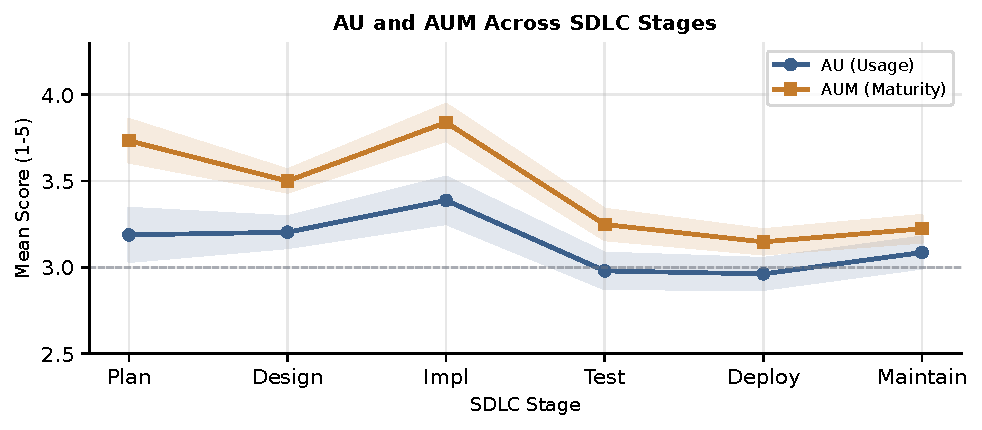
\includegraphics[width=\columnwidth]{fig1_au_aum_lines.pdf}
  \caption{Mean AU and AUM (with $\pm 1$ SE shading) across SDLC stages.
           AUM drops sharply after Implementation while AU remains
           comparatively flat, revealing a dissociation between usage
           frequency and usage quality.}
  \label{fig:lines}
\end{figure}

\subsubsection{AUM varies significantly across stages.}
A Friedman test on the complete-case subsample for \AUM ($N = 48$)
reveals a strong main effect of stage: $\chi^2(5) = 66.13$,
$p < .001$. Post-hoc Wilcoxon signed-rank tests with Bonferroni
correction for 15 pairwise comparisons (Table~\ref{tab:posthoc}) reveal
a clear two-cluster structure. Planning, Design, and Implementation
form a high-\AUM cluster ($M = 3.73$--$3.84$); Testing, Deployment,
and Maintenance form a low-\AUM cluster ($M = 3.15$--$3.25$). Every
early/middle vs.~late stage comparison except Design vs.~Testing is
significant after Bonferroni correction ($p < .05$), while no
pairwise comparison within either cluster survives correction.
Planning and Implementation, in particular, are statistically
indistinguishable in \AUM ($p = .85$), suggesting that the maturity of
AI interaction peaks early and carries through coding activities before
dropping sharply at testing.

\begin{table}[h]
\small
\caption{Pairwise Wilcoxon signed-rank post-hoc tests for AUM across
  SDLC stages (complete-case, $N = 48$). Bonferroni-corrected $p$
  values reported. {\bf **} $p<.01$; {\bf *} $p<.05$; n.s.~not
  significant.}
\label{tab:posthoc}
\begin{tabular}{llcc}
\toprule
\textbf{Stage A} & \textbf{Stage B} & $p_{\text{Bonf}}$ & \textbf{Sig.} \\
\midrule
Planning       & Design         & .026   & *    \\
Planning       & Implementation & 1.00   & n.s. \\
Planning       & Testing        & .001   & **   \\
Planning       & Deployment     & $<$.001 & ** \\
Planning       & Maintenance    & $<$.001 & ** \\
Design         & Implementation & .090   & n.s. \\
Design         & Testing        & .143   & n.s. \\
Design         & Deployment     & .004   & **   \\
Design         & Maintenance    & .005   & **   \\
Implementation & Testing        & .002   & **   \\
Implementation & Deployment     & $<$.001 & ** \\
Implementation & Maintenance    & $<$.001 & ** \\
Testing        & Deployment     & 1.00   & n.s. \\
Testing        & Maintenance    & 1.00   & n.s. \\
Deployment     & Maintenance    & 1.00   & n.s. \\
\bottomrule
\end{tabular}
\end{table}

\subsubsection{AU does not vary significantly across stages.}
In the same complete-case subsample for \AU ($N = 35$), the Friedman
test finds \emph{no significant difference in \AU across stages}:
$\chi^2(5) = 5.04$, $p = .41$. When sample composition is held
constant, students report broadly similar AI usage frequency across all
six \SDLC stages. This finding refines the common assumption---often
produced by between-subsample comparisons---that students use AI
substantially more in early stages. The contrast with the \AUM result
is striking: over the same lifecycle and same students, \emph{how}
they engage with AI varies enormously while \emph{how often} they
engage does not.

\subsection{Overall AU--AUM Relationship (RQ1)}
At the aggregate level, overall \AU and overall \AUM are strongly
positively correlated ($r = 0.690$, $p < .001$, $N = 85$), as shown in
Figure~\ref{fig:scatter}. Students who report more frequent AI use also
tend to engage in more mature usage practices.

\begin{figure}[h]
  \centering
  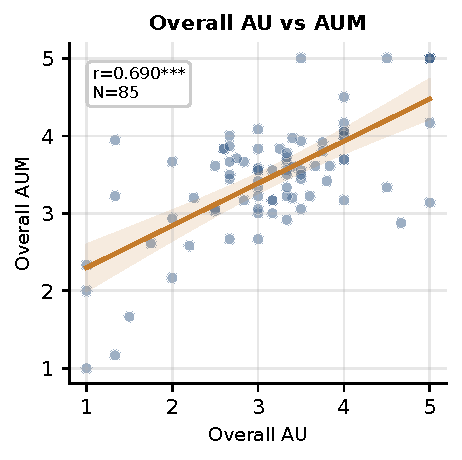
\includegraphics[width=0.85\columnwidth]{fig3_scatter.pdf}
  \caption{Overall AI Usage (AU) vs AI Usage Maturity (AUM) with
           regression line and 95\% confidence band ($r = 0.690$,
           $p < .001$, $N = 85$). Scatter around the line reveals
           meaningful individual-level variability.}
  \label{fig:scatter}
\end{figure}

\subsubsection{The AU--AUM coupling is stage-dependent.}
Figure~\ref{fig:corr} presents stage-level \AU--\AUM Pearson correlations.
Table~\ref{tab:corr} reports the full statistics. Three stages show a
statistically significant positive coupling: Planning ($r = 0.671$,
$p < .001$), Implementation ($r = 0.462$, $p < .001$), and Deployment
($r = 0.443$, $p = .001$). Three stages do not: Design ($r = 0.268$,
$p = .063$), Testing ($r = 0.278$, $p = .061$), and Maintenance
($r = 0.164$, $p = .224$).

\begin{figure}[h]
  \centering
  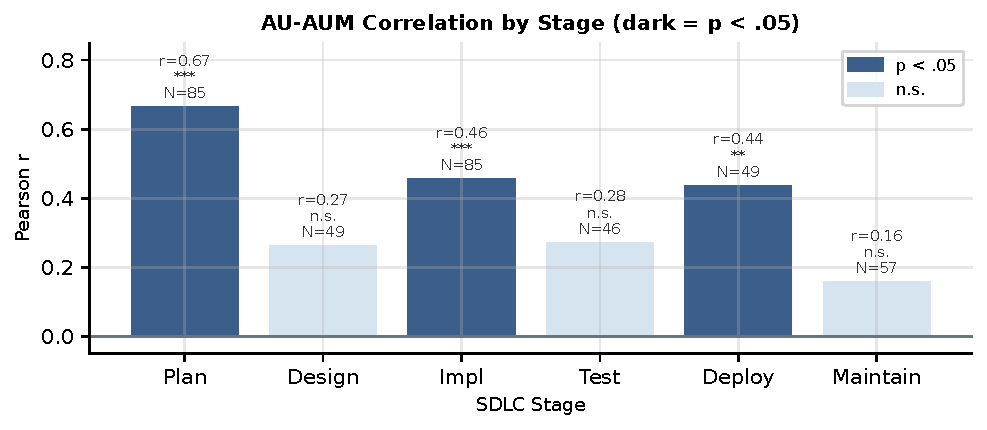
\includegraphics[width=\columnwidth]{fig2_corr_by_stage.pdf}
  \caption{Stage-level AU--AUM Pearson correlations. Dark bars indicate
           significant relationships ($p < .05$); light bars are
           non-significant. Planning shows the strongest coupling;
           Design, Testing, and Maintenance show no significant
           coupling.}
  \label{fig:corr}
\end{figure}

\begin{table}[h]
\small
\caption{Stage-level AU--AUM correlations.}
\label{tab:corr}
\begin{tabular}{lcccc}
\toprule
\textbf{Stage} & $r$ & $p$ & $N$ & \textbf{Sig.} \\
\midrule
Planning       & .671 & $<.001$ & 85 & *** \\
Design         & .268 & .063    & 49 & n.s. \\
Implementation & .462 & $<.001$ & 85 & *** \\
Testing        & .278 & .061    & 46 & n.s. \\
Deployment     & .443 & .001    & 49 & ** \\
Maintenance    & .164 & .224    & 57 & n.s. \\
\bottomrule
\multicolumn{5}{l}{\footnotesize *** $p<.001$; ** $p<.01$; n.s.\ not significant.}
\end{tabular}
\end{table}

\subsection{Stage-Level TAM Pathways: PU $\rightarrow$ AU}
While full \TAM pathway data are available only for Planning, the
stage-specific PU and AU items available for all six stages permit a
partial test of whether the PU $\rightarrow$ AU link in \TAM holds
uniformly across the \SDLC, or whether perceived usefulness predicts
usage more tightly at some stages than others. Table~\ref{tab:puau}
reports stage-level Pearson correlations between PU and AU. All six
correlations are positive and statistically significant
($p < .01$), confirming that perceived usefulness predicts self-reported
usage at every lifecycle stage. The magnitude, however, varies
substantially: PU$\rightarrow$AU is very strong at Planning
($r = .84$), moderate through Design ($r = .64$), Implementation
($r = .55$), and Maintenance ($r = .57$), and weaker but still
significant at Testing ($r = .46$) and Deployment ($r = .45$).

\begin{table}[h]
\small
\caption{Stage-level PU$\rightarrow$AU correlations. All
  correlations are significant at $p < .01$.}
\label{tab:puau}
\begin{tabular}{lccc}
\toprule
\textbf{Stage} & $r$ (PU, AU) & $p$ & $N$ \\
\midrule
Planning       & .839 & $<$.001 & 85 \\
Design         & .643 & $<$.001 & 50 \\
Implementation & .552 & $<$.001 & 85 \\
Testing        & .460 & .002    & 43 \\
Deployment     & .447 & .001    & 49 \\
Maintenance    & .568 & $<$.001 & 55 \\
\bottomrule
\end{tabular}
\end{table}

The attenuation of PU$\rightarrow$AU at later stages is theoretically
informative. In classical \TAM, the PU $\rightarrow$ AU pathway reflects
the degree to which believing a tool is useful translates into actually
using it. A weaker PU$\rightarrow$AU link at Testing and Deployment
suggests that, in those stages, students' actual AI use is decoupled
from how useful they judge AI to be for the task. Taken together with
the non-significant \AU--\AUM coupling at those same stages
(Table~\ref{tab:corr}), this points to a consistent pattern at
late-\SDLC stages: AI use at Testing, Deployment, and Maintenance
appears to be opportunistic and weakly regulated by either perceived
utility or disciplined practice.

\subsection{TAM Constructs and Antecedents}
Full \TAM data (PEOU, PU, BI, AU) are available for the Planning stage.
Figure~\ref{fig:heatmap} shows the full correlation matrix. \TAM
intercorrelations are uniformly strong (PU--BI: $r = .88$; PU--AU:
$r = .85$; PEOU--PU: $r = .74$), consistent with prior \TAM validation
studies~\cite{ali2025, simsek2025}. Planning-stage AU correlates
strongly with overall \AU ($r = .80$), suggesting that early-stage
behavior is predictive of lifecycle-wide engagement patterns.

AI Literacy correlates with overall \AU ($r = .14$, $p = .27$, n.s.)
and more strongly with overall \AUM ($r = .35$, $p = .004$).
Facilitating Conditions shows a moderate relationship with overall \AU
($r = .46$, $p < .001$). This asymmetry is theoretically meaningful:
access to tools (Facilitating Conditions) predicts \emph{whether}
students use AI, while literacy predicts \emph{how well} they use it.
In a cohort where tool access is effectively universal, the remaining
variation in mature AI use is better explained by cognitive and
evaluative skills than by infrastructure availability.

\begin{figure}[h]
  \centering
  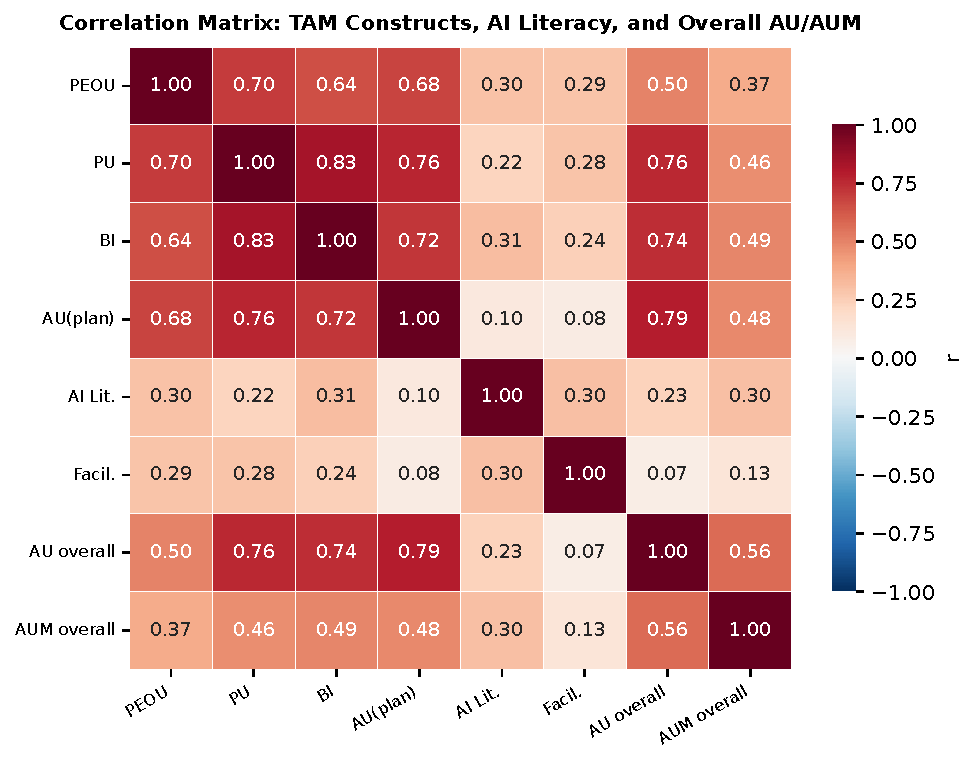
\includegraphics[width=\columnwidth]{fig4_heatmap.pdf}
  \caption{Correlation matrix of Planning-stage \TAM constructs, AI
           Literacy, Facilitating Conditions, and overall AU/AUM.
           Strong \TAM intercorrelations replicate prior findings.}
  \label{fig:heatmap}
\end{figure}

%% ==========================================================================
\section{Discussion}
\label{sec:discussion}

\subsection{Differential Non-Response as a Substantive Finding}
The fact that 59\% of respondents did not complete all stage sections may
itself reflect genuine disengagement with later \SDLC phases in the
actual course project. Students who did not actively engage with
deployment or maintenance had little to report. This interpretation is
consistent with the lower \AUM scores for those stages. Future work
should use longitudinal or repository-based data to distinguish between
incomplete survey sections and incomplete \SDLC engagement.

\subsection{Revisiting the Research Questions}
We now return to the two research questions that motivated this study
and use the empirical patterns to state what each finding means for
practitioners.

\textbf{RQ1: How does AI usage relate to AI usage maturity across SDLC
stages?} At the overall level, the answer is clear---\AU and \AUM are
strongly correlated ($r = .69$). But this aggregate hides three
distinct stage-level regimes. Three stages show a \emph{significant
positive AU--AUM coupling}: Planning ($r = .67$), Implementation
($r = .46$), and Deployment ($r = .44$). In these stages, students who
use AI more also use it more maturely. Three stages show \emph{no
significant coupling}: Design ($r = .27$), Testing ($r = .28$), and
Maintenance ($r = .16$). In these stages, usage frequency tells us
nothing about usage quality. The heterogeneity is itself the finding:
any educational response must be stage-specific.

\textbf{RQ2: How does AI usage maturity vary across SDLC stages?}
Very substantially, and in a structured way. \AUM separates cleanly
into a high cluster (Planning, Design, Implementation; $M \approx 3.8$)
and a low cluster (Testing, Deployment, Maintenance;
$M \approx 3.2$), with essentially every cross-cluster pairwise
comparison significant after Bonferroni correction
(Table~\ref{tab:posthoc}). Students have---on average---developed
disciplined AI practices for the first half of the \SDLC and have not
yet developed them for the second half. Meanwhile \AU is flat across
the same stages. This is, to our knowledge, the first empirical
demonstration in a CS educational setting that AI usage quality and
AI usage frequency follow different lifecycle profiles.

\subsection{What Should Instructors Actually Do?}
Combining the RQ1 and RQ2 patterns with the stage-level PU$\rightarrow$AU
correlations (Table~\ref{tab:puau}), four concrete instructional
priorities follow. These are keyed to specific empirical patterns
rather than to the general observation that AI matters.

\textbf{1. Use the Planning stage to seed mature practices.} Planning
shows the strongest PU$\rightarrow$AU coupling ($r = .84$), the
strongest AU--AUM coupling ($r = .67$), and the strongest planning-AU
$\rightarrow$ overall-AU correlation ($r = .80$). These three
findings together tell a coherent story: how students engage with AI
during planning predicts their lifecycle-wide AI behavior more than
any other stage we measured. Instructors who want to shape AI habits
should intervene at the planning stage with explicit scaffolds---for
example, requiring students to document the structured goals and
constraints they gave to AI, and having them defend planning outputs
in a sprint review before proceeding to design.

\textbf{2. Change the structure of later-stage AI use, not just its
frequency.} The low-\AUM cluster (Testing, Deployment, Maintenance)
combines low maturity, attenuated PU$\rightarrow$AU coupling, and
near-zero or non-significant AU--AUM coupling. This means students at
these stages use AI opportunistically without either a clear sense of
why AI is useful or a structured way of using it. Adding more AI
prompts or examples will not fix this---it will raise \AU without
raising \AUM. What is needed is structural scaffolding: for testing,
require students to specify a test-generation prompt, document the
failure analysis loop, and record which AI-generated tests they
accepted and why; for deployment, pair AI-suggested CI/CD changes with
a required staging log review; for maintenance, require students to
frame AI as a hypothesis generator whose suggestions must be verified
against regression results.

\textbf{3. Teach literacy, not tool access.} In this cohort tool
access is effectively universal (89\% weekly \GenAI users; 42\% use
Claude, 34\% use ChatGPT), and Facilitating Conditions correlates more
strongly with \AU than with \AUM ($r = .46$ vs $r = .20$). AI
Literacy---critical evaluation, ethical competence, interpreting
limitations---correlates more strongly with \AUM than with \AU
($r = .35$ vs $r = .14$). For experienced, AI-fluent students, adding
more tools or more access will not improve the quality of AI use. What
will improve quality is direct instruction on evaluating, critiquing,
and verifying AI outputs---topics that fit naturally into existing
course units on code review, testing, and software quality.

\textbf{4. Address heterogeneity within cohorts, not just between
stages.} Even in Implementation, where \AUM is highest on average, a
subset of students report minimal AI use and another subset report
heavy use with low maturity. Classroom practices that assume uniform
AI engagement will miss both tails. Differentiated prompts, AI-use
self-assessments, and tiered scaffolding---where students with low
\AUM receive structured templates while students with higher \AUM
receive critique-focused exercises---can address this within-stage
heterogeneity that our aggregated means do not expose.

%% ==========================================================================
\section{Limitations and Future Work}
\label{sec:limitations}

This study has several important limitations. First, all measures are
self-reported; students may systematically overreport mature practices,
particularly in a course context where such behaviors are valued. Social
desirability bias is a known concern in educational surveys, and our use
of five-point Likert scales does not mitigate this directly. Future
triangulation with observable artifacts---prompt logs, commit histories,
or code review records---would help validate self-report measures.

Second, the sample is drawn from a single institution and two sections
of the same course, which limits generalizability. Students in this
cohort are relatively experienced (80\% with $\geq 3$ years of
programming) and AI-fluent (89\% weekly users), and results may differ
substantially in courses with novice learners or restricted tool access.
Third, the team-based project structure means individual responses may
not be independent, since team members may influence each other's AI
usage practices. A multilevel modeling approach incorporating team-level
random effects would be appropriate in a larger sample.

Fourth, the differential non-response across stages introduces
uncertainty about whether stage-level \AUM differences reflect genuine
behavioral patterns or selective survey completion. While we report
complete-case analyses to mitigate this concern, future studies should
employ within-session reminders or shorter per-stage item sets to
reduce stage-level attrition.

Future work should link self-reported \AU and \AUM to observable
software artifacts, examining whether \AUM differences correspond to
measurable differences in code quality, maintainability, or project
outcomes. Static analysis and AST-based repository mining offer
promising approaches for bridging this gap. Longitudinal designs could
also examine whether students' \AUM evolves over time as they gain
experience with AI tools across multiple projects and courses,
and whether targeted pedagogical interventions can shift \AUM at
specific \SDLC stages---particularly testing, deployment, and
maintenance, where the current data suggest the greatest opportunity
for improvement.

%% ==========================================================================
\section{Conclusion}
\label{sec:conclusion}

This study advances a stage-aware perspective on \GenAI adoption in
software engineering education through an empirical analysis of 85
undergraduate students. Three findings stand out. AI usage frequency
does not differ significantly across \SDLC stages when sample
composition is held constant. AI usage maturity does differ
(Friedman $\chi^2 = 66.13$, $p < .001$), with Planning, Design, and
Implementation showing meaningfully higher \AUM than Testing,
Deployment, and Maintenance. The coupling between the two is itself
stage-dependent: tightest in Planning ($r = .671$) and absent in
Maintenance ($r = .164$, n.s.). Together with the stage-level
PU$\rightarrow$AU evidence, these patterns support a stage-aware
perspective on AI adoption and provide educators with a practical
framework---grounded in specific correlations rather than general
intuitions---for assessing the quality of AI-assisted development
practices across the full software lifecycle.

%% ── Acknowledgements ──────────────────────────────────────────────────────
\begin{acks}
[Acknowledgements omitted for double-blind review.
Space reserved for funding, course staff, and student participants.]

\medskip\noindent\textbf{AI Disclosure.} In accordance with ACM policy on
authorship, the authors disclose that Claude (Anthropic) was used to
support writing assistance and data analysis scripting during the
preparation of this manuscript. All research questions, theoretical
framing, empirical analysis decisions, interpretation of results, and
conclusions are the sole responsibility of the authors.
\end{acks}

%% ==========================================================================
%% REFERENCES — optional page 7 (references only, no other content)
%% SIGCSE: references may occupy an optional 7th page; appendices not
%% permitted on that page. All body content must remain within 6 pages.
%% ==========================================================================
\newpage
\bibliographystyle{ACM-Reference-Format}
\bibliography{refs}

\end{document}
